%%%%%%%%%%%%%%%%%%%%%%%%%%%%%%%%%%%%%%%%%%%%%%%%%%%%%%%%%%%
% --------------------------------------------------------
% Tau
% LaTeX Template
% Version 2.4.1 (22/05/2024)
%
% Author: 
% Guillermo Jimenez (memo.notess1@gmail.com)
% 
% License:
% Creative Commons CC BY 4.0
% --------------------------------------------------------
%%%%%%%%%%%%%%%%%%%%%%%%%%%%%%%%%%%%%%%%%%%%%%%%%%%%%%%%%%%
\documentclass[9pt,a4paper,twoside]{tau-class/tau}

%----------------------------------------------------------
% TITLE
%----------------------------------------------------------

\usepackage{enumitem}
\newcount\NewCount

\journalname{ESCOM}
\title{Cellular Automata}


%----------------------------------------------------------
% AUTHORS, AFFILIATIONS AND PROFESSOR
%----------------------------------------------------------

\author[a]{Diego Castillo Reyes}
\author[a]{Marthon Leobardo Yañez Martinez}
\author[a]{Aldo Escamilla Resendiz}
\author[a]{Muñoz González Eduardo}

%----------------------------------------------------------

\affil[a]{Researcher}


\professor{Dra. Miriam Pescador Rojas}

%----------------------------------------------------------
% FOOTER INFORMATION
%----------------------------------------------------------

\institution{Escuela Superior de Cómputo, IPN}
\footinfo{Cellular Automata}
\theday{June 21, 2024}
\course{Genetic Algorithms}

%----------------------------------------------------------
% ABSTRACT AND KEYWORDS
%----------------------------------------------------------

\begin{abstract}    
    Cellular automata are a mathematical and computational model used to simulate dynamic systems. 
        This work presents a review of cellular automata, their history, classification, and applications. 
        Additionally, an example of one-dimensional and two-dimensional cellular automata is shown.
\end{abstract}

%----------------------------------------------------------

\keywords{Automata, Cellular, Genetic, Algorithms, Simulation}

%----------------------------------------------------------

\begin{document}	
    \maketitle 
    \thispagestyle{firststyle} \tauabstract
    \tableofcontents
%----------------------------------------------------------

\section{Introduction}

    Cellular automata (CA) are \textit{discrete, abstract computational systems} that have proved useful both as general models of complexity and as more specific representations of non-linear dynamics in a variety of scientific fields. 

    Firstly, CA are typically spatially and temporally discrete. They are composed of a finite or denumerable set of homogeneous, simple units called cells. At each time unit, the cells instantiate one of a finite set of states. 
    They evolve in parallel at discrete time steps, following state update functions or dynamical transition rules. 
    The update of a cell's state is obtained by taking into account the states of cells in its local neighborhood, meaning there are no actions at a distance.

    Secondly, CA are abstract. They can be specified in purely mathematical terms, and physical structures can implement them.

    Thirdly, CA are computational systems. They can compute functions and solve algorithmic problems. Despite functioning differently from traditional 
    Turing machine-like devices, CA with suitable rules can emulate a universal Turing machine\footnote{\cite[The Stanford Encyclopedia of Philosophy (Winter 2021 Edition), Edward N. Zalta (ed.)]{sep-touring-machine}}, 
    and therefore compute anything that is computable according to Turing's thesis.\cite{sep-cellular-automata}


\section{Background}


    The concept of cellular automata was invented by Stansilaw Ulam and John Von Neumann in
    the 1940s while they were working at the Los Alamos National Laboratory.
    The work on cellular automata began in the 1940s, with significant developments occuring throughout
    that decade. Von Neumann’s comprehensive work on self-replicating automata was published 
    posthumously in 1966 in the book ``Theory of Self-Reproducing Automata'', edited by 
    Arthur W. Burks.

    A cellular automaton (CA) is a one-dimensional array (which can be infinitely long in both directions) of cells. 
    Time progresses in discrete steps, and at each step, every cell is in one of a finite number of possible states. The state of each cell changes at each tick of the clock, and this new state is determined entirely by the current state of the cell and its immediate left and right neighbors. 
    This state change is governed by a function called the local rule, which is identical for all cells. 
    The CA operates autonomously without any external input. 
    The collection of all cell states at any given time is referred to as the configuration or global state of the CA, 
    representing its stage of evolution. Starting from an initial configuration at time t = 0, the CA evolves deterministically according to the local 
    rule applied to each cell at each clock tick. (see Fig. \ref{fig:timeStep})

    When the local rule is applied to each cell, it transforms the entire set of configurations into itself. 
    This transformation is known as the global map or global rule of the CA. This description captures the essence of a CA, which is a widely studied structure.
    \begin{figure}[H]
        \centering
        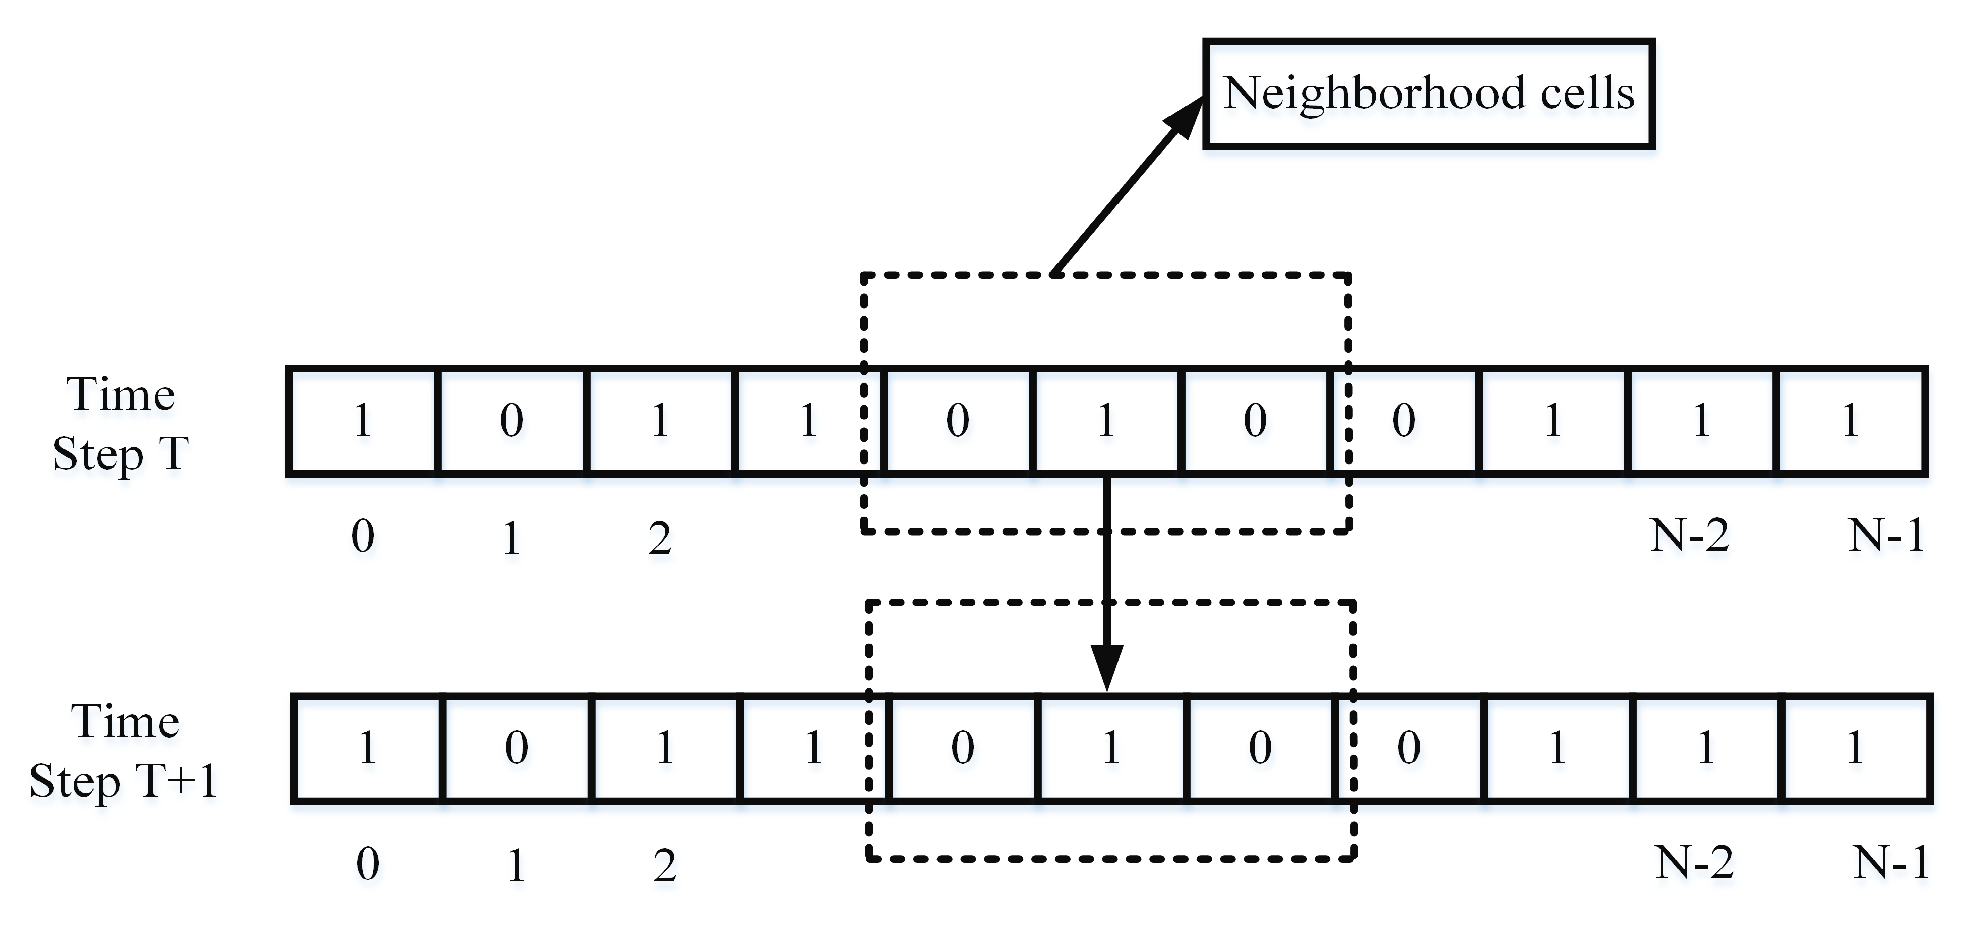
\includegraphics[width=0.75\columnwidth]{figures/timestep.png}
        \caption{Evolution of a CA at each time step. \cite{math11102322}}
        \label{fig:timeStep}
    \end{figure}

    The automaton initially described by von Neumann\cite{von-neumann-automata} consists of a two-dimensional infinite array of uniform cells, with each cell connected to its four orthogonal neighbors. 
    This structure was originally termed a cellular space, though the term CA is now more commonly used. Von Neumann introduced this concept as a formal model for self-reproducing biological systems. His key ideas can be traced back to his earlier work on modeling biological systems. 
    Von Neumann aimed to apply the rigor of axiomatic and deductive methods to the study of complex natural systems. His concept of a self-reproducing automaton is a remarkable adaptation of the idea behind constructing a universal Turing Machine (TM).

    \begin{figure}[H]
        \centering
        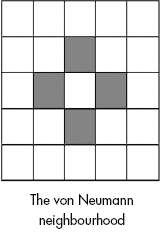
\includegraphics[width=0.75\columnwidth]{figures/vonNeumann.png}
        \caption{Von Neumann's cellular automaton.}
        \label{fig:vonNeumann}
    \end{figure}


    \subsection{One-Dimensional Cellular Automata}


    Most of the dynamic features of cellular automata can be observed in the study of the one-dimensional case. In this context, we define the neighborhood of a cell \( c \) with a radius \( r \) as the \( r \) cells to the left of \( c \) and the same number of cells to the right of \( c \). Including \( c \) itself, this neighborhood comprises \( 2r + 1 \) cells. For the simplest case where \( r = 1 \) and \( k = 2 \) (the allowable states), a three-cell neighborhood with two possible states (0 and 1) for each cell can be expressed in \( 2^3 = 8 \) different ways. All eight neighborhood states with \( r = 1 \) and \( k = 2 \) are illustrated in Figure \ref{fig:neighborhood_states}, and in general, there are \( k^{2r+1} \) one-dimensional neighborhood states.\cite{schiff2007}
    
        \begin{figure}[H]
            \centering
            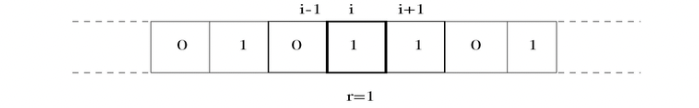
\includegraphics[width=0.9\columnwidth]{figures/transition_rule.png}
            \caption{Eight possible neighborhood states with \( r = 1 \) and \( k = 2 \).}
            \label{fig:neighborhood_states}
        \end{figure}
    Let us adopt the notation \( c_i(t) \) to denote the state of the \( i \)-th cell at time \( t \) (Figure \ref{fig:cell_states}).
    
    
    \begin{figure}[H]
        \centering
        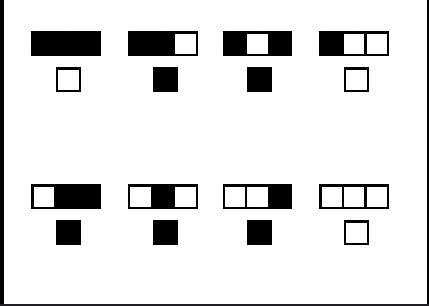
\includegraphics[width=0.45\columnwidth]{figures/rule_graphic.png}
         \caption{State of the \( i \)-th cell at time \( t \).} 
        \label{fig:cell_states}
    \end{figure}


    At the next time step, \( t + 1 \), the cell state will be \( c_i(t + 1) \). Mathematically, we can express the dependence of a cell’s state at time step \( t + 1 \) on the states of its left and right nearest neighbors \( c_{i-1}(t) \) and \( c_{i+1}(t) \) at time step \( t \) by the relation

    \begin{equation}
        c_i(t + 1) = \phi \left( c_{i-1}(t), c_i(t), c_{i+1}(t) \right),
    \end{equation}

    where \( \phi \) is the local transition function. For example, consider the simple transition rule

    \begin{equation}
        c_i(t + 1) = \left( c_{i-1}(t) + c_i(t) + c_{i+1}(t) \right) \mod 2,
        \label{eq:transition_rule}
    \end{equation}

    where $\mod 2$ means taking the remainder after dividing the indicated sum by 2, resulting in either 0 or 1. We can put this rule into a transition table format by computing \( c_{i-1}(t) + c_i(t) + c_{i+1}(t) \mod 2 \) for the eight possible input values:

    \begin{table}[H]
        \centering
        \begin{tabular}{cccc}
            \toprule
            $c_{i-1}(t)$ & $c_i(t)$ & $c_{i+1}(t)$ & $c_i(t + 1)$ \\
            \midrule
            1 & 1 & 1 & 1 \\
            1 & 1 & 0 & 0 \\
            1 & 0 & 1 & 0 \\
            1 & 0 & 0 & 1 \\
            0 & 1 & 1 & 0 \\
            0 & 1 & 0 & 1 \\
            0 & 0 & 1 & 1 \\
            0 & 0 & 0 & 0 \\
            \bottomrule
        \end{tabular}
        \caption{Transition table for the rule \( c_i(t + 1) = (c_{i-1}(t) + c_i(t) + c_{i+1}(t)) \mod 2 \).}
        \label{tab:transition_table}
    \end{table}

    A very convenient way to illustrate the allowable rules for one-dimensional cellular automata with \( r = 1 \) and \( k = 2 \) is to indicate the state (color) of the middle cell at the next time step, given the state (color) of itself and its two nearest neighbors (Figure \ref{fig:cell_states}).

    Here, the middle cell at time \( t \) (in the top row) has its state altered according to the states of its two nearest neighbors and its own state to yield the cell’s new state at time \( t + 1 \) (bottom row). This also represents the rule in Equation \ref{eq:transition_rule}. Observe that in four of the eight cases, a black cell appears. One consequence of this is that if we took a disordered array of a large number of cell sites, then the average fraction (or density) of black cell sites that evolve after one iteration will be 0.5.

    The cellular automaton defined by this rule has the graphical representation depicted in Figure \ref{fig:rule_graphic}, starting with a single black cell with each subsequent generation of the automaton appearing on the next line down.
    \begin{figure}[H]
        \centering
        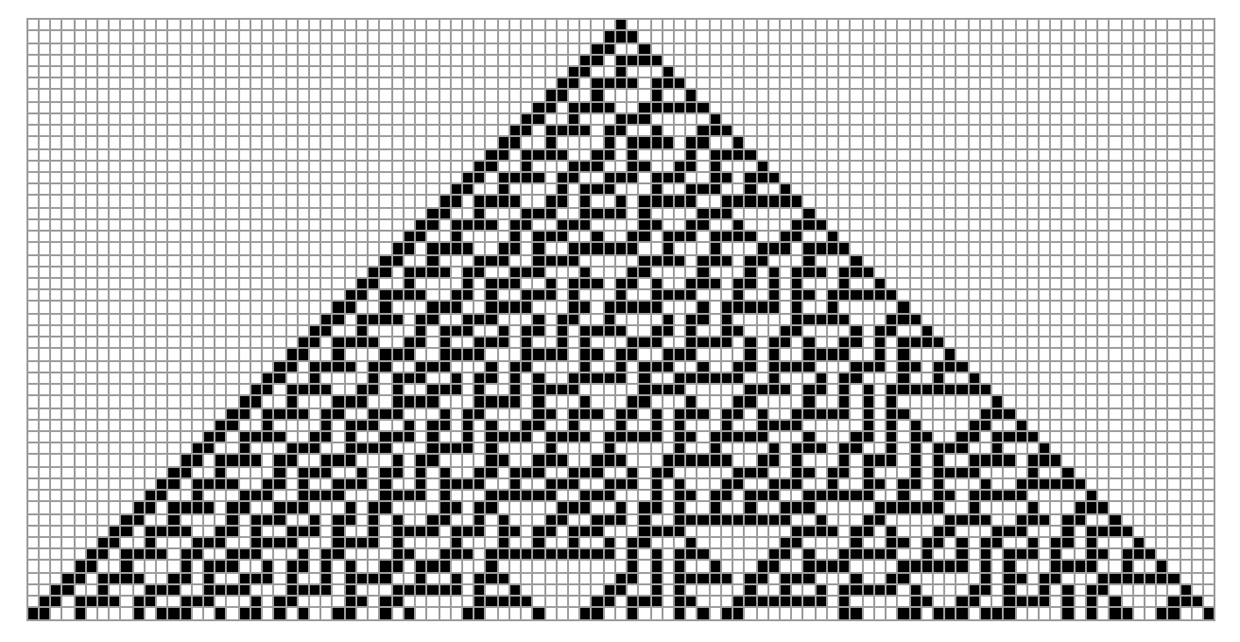
\includegraphics[width=0.75\columnwidth]{figures/rule30.png}
         \caption{Graphical representation of the evolution of the rule starting with a single black cell. Each new line downward represents the evolution of the automaton at the next time step.} 
        \label{fig:rule_graphic}
    \end{figure}

    So, how many possible rules are there for \( r = 1 \) and \( k = 2 \)? Since there are eight possible neighborhood states of three cells and each of these results in two possible state outcomes for the middle cell, there are \( 2^8 = 256 \) possible transition rules by which this can be achieved as seen in Figure~\ref{fig:floatrules}. Wolfram described these as elementary cellular automata.

    \begin{figure*}[tp] % t for position at the top of the current page; b for position at the bottom; p for new page
		\centering
		  \begin{subfigure}[b]{0.38\linewidth} % Fig (a)
			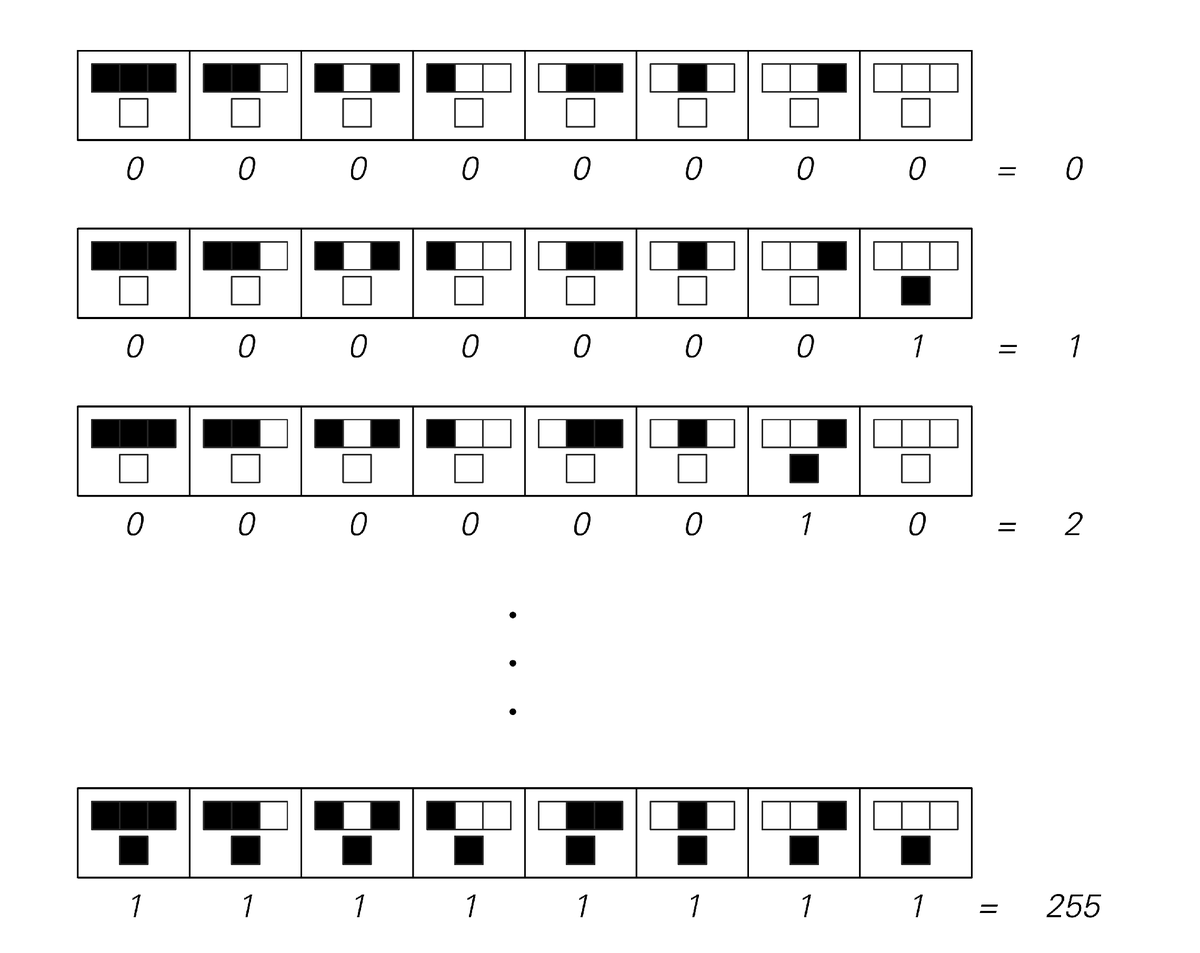
\includegraphics[width=\linewidth]{figures/rules256.png}
			\caption{The 256 rules}
		\end{subfigure}
			\hspace{20pt}   % Space between the figures
		\begin{subfigure}[b]{0.375\linewidth} % Fig (b)
			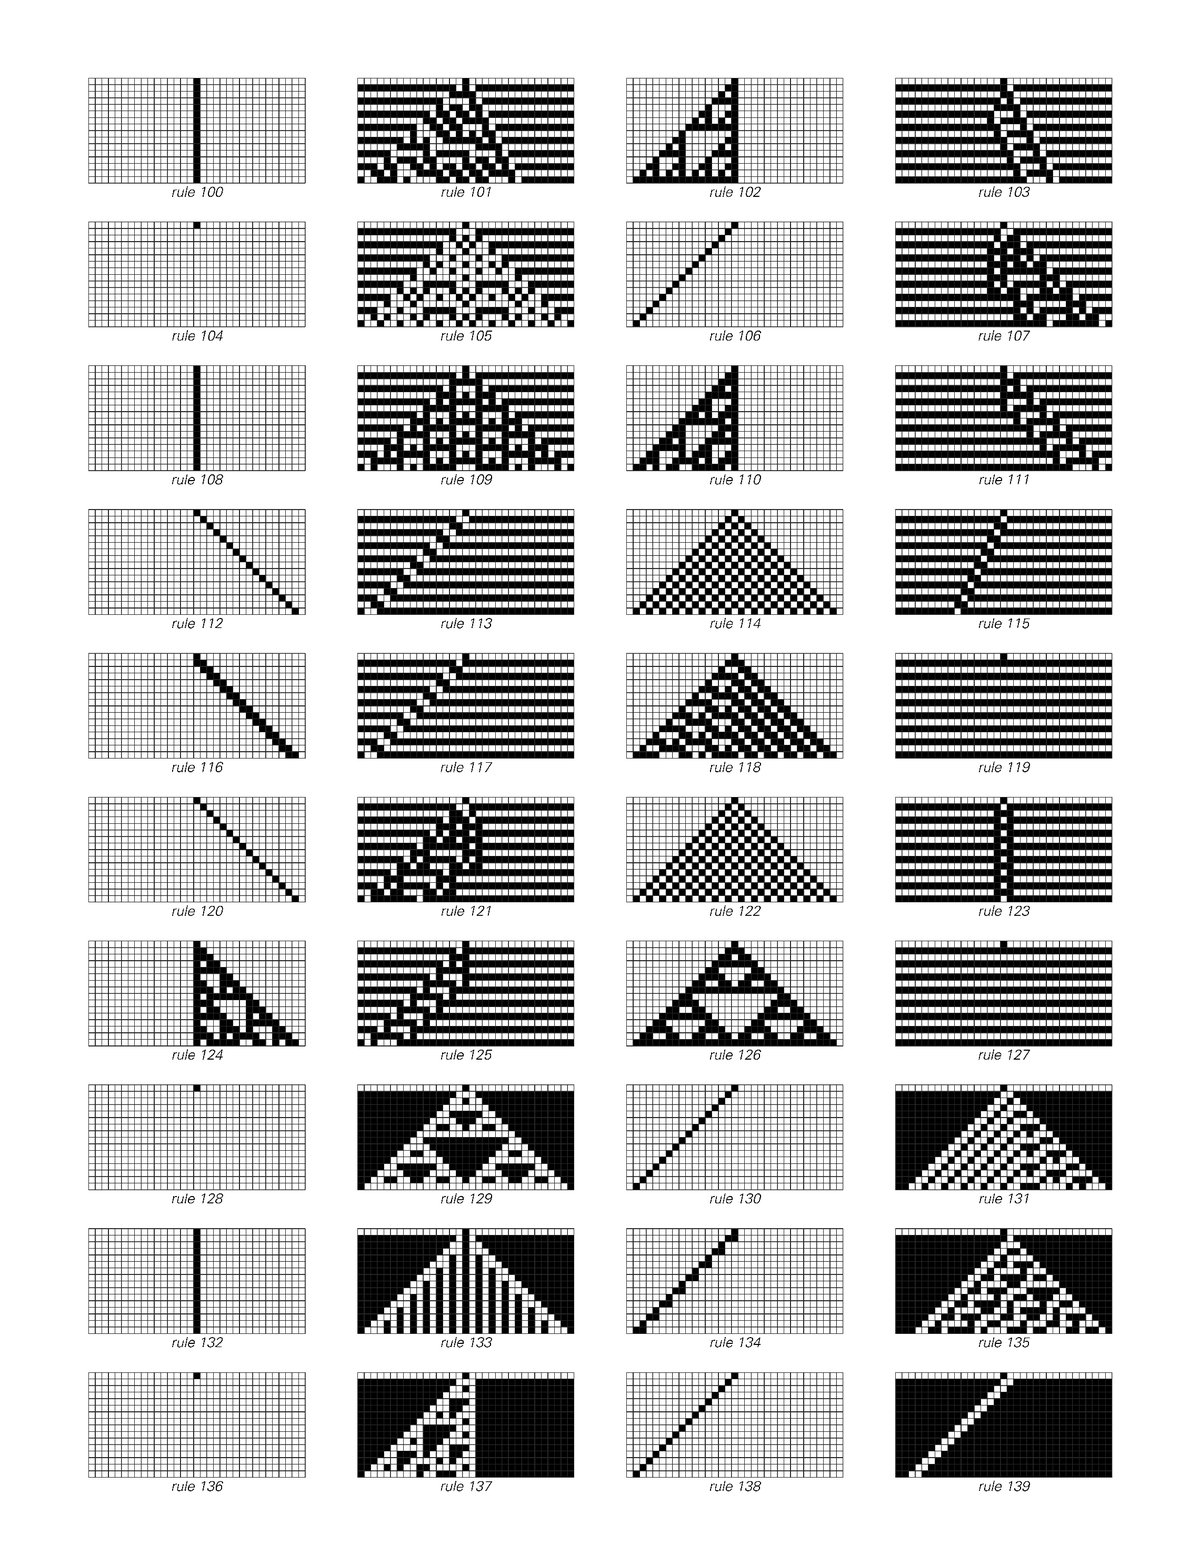
\includegraphics[width=\linewidth]{figures/generetions.png}
			\caption{Genereations for some rules}
		\end{subfigure}
		\caption{The 256 rules and the generations for some of them.}
		\label{fig:floatrules}
	\end{figure*}

    \subsection{Motivation}
    
    
    Cellular automata, a concept derived from computer science, are increasingly employed as models in ecological research. This concept spans a variety of topics, including automata theory and artificial intelligence. 
    Cellular automata, as representations of this concept, create miniature worlds where each cell houses an automaton. The behavior of a cellular automaton can be remarkably complex, often resembling lifelike processes. 
    This complexity has inspired a new field of study known as artificial life or, more cautiously, complex systems. Conferences in this field attract computer and mathematical scientists, as well as a growing number of participants from geography, ecology, geology, and other disciplines, along with a popular audience. 
    Currently, the field of ecology has accumulated sufficient experience with cellular automaton models to move beyond initial simple models and harness the full potential of this tool for comprehensive simulation. 
    However, validation and interpretation continue to be significant challenges in utilizing these models effectively.\cite{DEWDNEY2008541}

    The primary motivation behind cellular automata was to understand and model complex
    systems using simple, local rules. This idea was rooted in the study of biological 
    processes and the desire to create self-replicating machines.

    \subsection{Developments}
  
    John Conway's work (1970s): Conway popularized cellular
    automata with his "Game of Life", a bidimensional binary cellular automaton. 
    This game demonstrated how simple rules could lead to complex emergent behavior, 
    sparking widespread interest and research in cellular automata.


    Fig. \ref{fig:figure} An example of Conway's Game of Life.
	\begin{figure}[H]
		\centering
		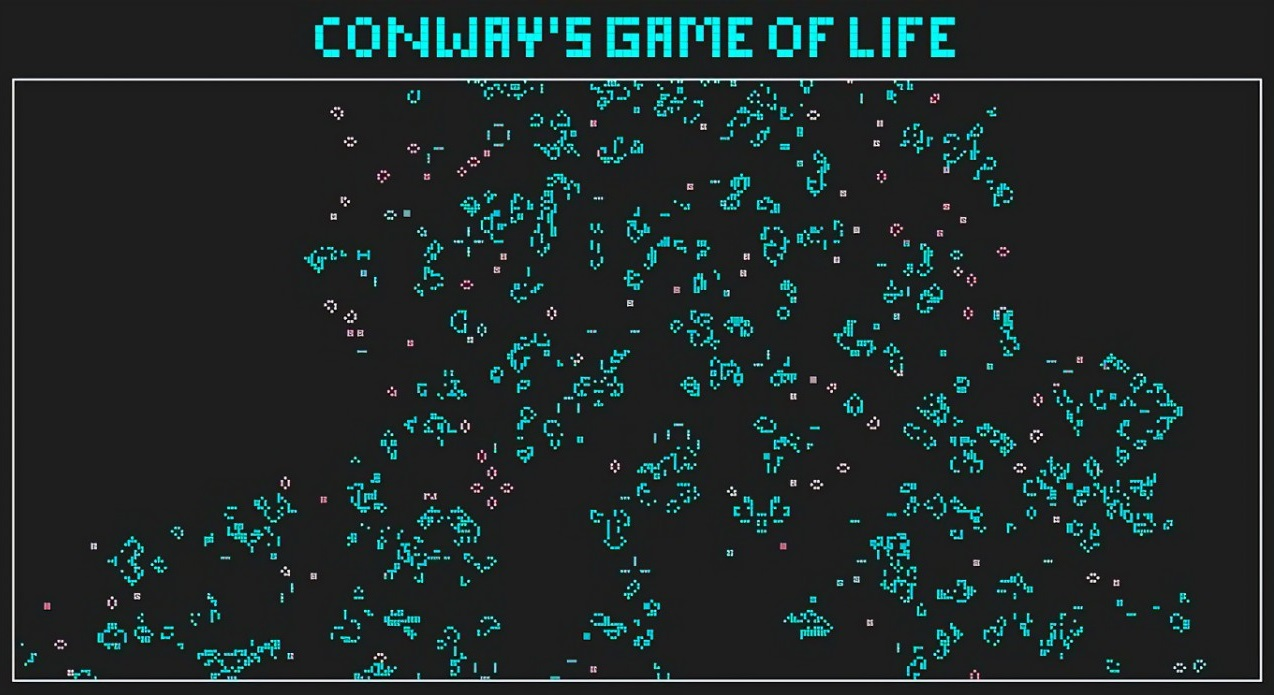
\includegraphics[width=0.75\columnwidth]{figures/gameOfLife.jpg}
		\caption{Conway's Game of Life.}
		\label{fig:figure}
	\end{figure}

    Stephen Wolfram's work (1980s): Wolfram conducted extensive research on cellular
    automata, classifying them into four types based on their behavior and demonstrating 
    their potential as models of natural processes and as computational systems.
  
    \subsubsection{John Conway's Game of Life}


    John Conway's Game of Life is a well-known example of a two-dimensional cellular automaton. Devised by the British mathematician John Horton Conway in 1970, it gained significant interest due to its simplicity and the complex behaviors it can exhibit.

    \subsubsection{Rules of the Game}

    The Game of Life is played on a rectangular grid of cells, where each cell can be in one of two states: alive (1) or dead (0). The state of each cell evolves through discrete time steps according to a set of simple rules based on the states of its eight neighbors (the Moore neighborhood). A dead cell with exactly three live neighbors becomes a live cell, akin to reproduction. A live cell with two or three live neighbors remains alive, reflecting a stable environment. Conversely, a live cell with fewer than two live neighbors dies, simulating underpopulation, and a live cell with more than three live neighbors dies, simulating overpopulation.

    \subsubsection{Initial Configuration and Evolution}

    The evolution of the grid begins from an initial configuration of live and dead cells. The subsequent generations are determined by simultaneously applying the aforementioned rules to every cell in the grid. This process is repeated for as many time steps as desired, creating a dynamic and evolving pattern.

    \subsubsection{Emergent Patterns}

    One of the most fascinating aspects of the Game of Life is the emergence of complex patterns from simple initial conditions. Still lifes, such as the Block and Beehive, are patterns that do not change from one generation to the next. Oscillators, like the Blinker and Toad, return to their initial state after a fixed number of generations. Spaceships, including the Glider and Lightweight Spaceship (LWSS), translate themselves across the grid, demonstrating movement.

    \subsubsection{Significance and Applications}

    The Game of Life has been extensively studied not only as a mathematical curiosity but also for its implications in various fields. In computational theory, the Game of Life is Turing complete, meaning it can simulate any computation given enough resources, demonstrating that simple rules can lead to universal computation\cite{rendell2002turing}. In the study of complex systems, it serves as a model for emergent behavior, illustrating how simple interactions can lead to intricate and unpredictable patterns \cite{gardner1970}. Researchers in artificial life use the Game of Life to study processes such as self-replication, evolution, and the emergence of life-like properties from non-living systems \cite{langton1986}.

    \subsubsection{Simulation and Visualization}

    The Game of Life is often simulated using computers to explore its vast array of patterns and behaviors. Many software tools and libraries have been developed for this purpose. Golly is a popular open-source application that allows users to create, simulate, and analyze patterns in the Game of Life and other cellular automata\cite{golly}. Various online platforms also enable users to interactively explore the Game of Life directly in their web browsers, making it accessible for educational and research purposes.

    \subsubsection{Conclusion}

    John Conway's Game of Life exemplifies the power and elegance of cellular automata. Its simple rules lead to complex and fascinating behaviors, making it a rich subject for study in mathematics, computer science, and beyond. The Game of Life continues to inspire and challenge researchers, illustrating the profound connection between simplicity and complexity in dynamic systems.

    \subsection{Stephen Wolfram's Research on Cellular Automata}

    Stephen Wolfram is a prominent figure in the study of cellular automata, and his research has significantly advanced the understanding of these systems. Wolfram's work explores the complexity that arises from simple rules and how such systems can model natural phenomena.\cite{wolfram1983}

    \subsubsection{Elementary Cellular Automata}

    Wolfram's research primarily focuses on one-dimensional cellular automata, known as elementary cellular automata. These consist of a line of cells, each of which can be in one of two states: 0 (dead) or 1 (alive). The state of each cell in the next time step depends on its current state and the state of its two immediate neighbors. Despite the simplicity of these rules, elementary cellular automata can exhibit a wide range of behaviors, from predictable and repetitive to highly complex and chaotic.

    \subsubsection{Rule Classification}

    Wolfram classified the behavior of cellular automata into four classes based on their long-term behavior:\cite{wolfram1984}

    \textbf{Class 1:} These automata evolve into a homogeneous state. Any random initial configuration eventually leads to a uniform state. This behavior is similar to systems that settle into a stable equilibrium.

    \textbf{Class 2:} These automata evolve into a set of stable or oscillating structures. Patterns emerge that are stable or repeat periodically. This behavior is akin to the formation of stable structures or cycles in nature.

    \textbf{Class 3:} These automata produce random or chaotic patterns. Small changes in the initial configuration can lead to significant differences in the evolution of the automaton, reflecting chaotic systems in nature.

    \textbf{Class 4:} These automata generate complex structures that can interact with each other in complicated ways. This class is particularly interesting because it can support universal computation, meaning these automata can perform any computation given the right initial conditions and rules.

    \subsubsection{Rule 30 and Rule 110}

    Among the elementary cellular automata, Rule 30 and Rule 110 are particularly notable. Rule 30 generates a pattern that appears random and is used in random number generation.\cite{wolfram2002}\cite{cook2004} It exhibits chaotic behavior from simple initial conditions. Rule 110, on the other hand, has been proven to be Turing complete, meaning it can simulate any computation. This demonstrates that even simple rules can lead to computational universality.

    \subsubsection{Applications and Implications}

    Wolfram's research has broad implications across various fields. In physics, cellular automata provide models for understanding complex systems and phenomena such as fluid dynamics and pattern formation. In computer science, they offer insights into computation theory and the nature of complexity. Wolfram's work also intersects with biology, where cellular automata can model the growth patterns of organisms and the dynamics of ecosystems.

    \subsubsection{A New Kind of Science}

    Wolfram's seminal book, \textit{A New Kind of Science}, encapsulates his research and presents a comprehensive view of how simple computational rules can lead to complex behaviors. The book argues that the universe itself might operate according to principles similar to those of cellular automata, suggesting a computational foundation for all natural processes.

    \subsubsection{Conclusion}

    Stephen Wolfram's research on cellular automata reveals the profound complexity that can arise from simple rules. His classification of automata behaviors, the study of specific rules like Rule 30 and Rule 110, and the broader implications for understanding natural phenomena highlight the importance of cellular automata in both theoretical and applied sciences. Wolfram's work continues to inspire researchers and offers a unique perspective on the computational nature of the universe.





    \subsection{Applications}
	
        Cellular automata have been used in various fields, including:
        
        \begin{itemize}
            \item Computer Science: Parallel computation, cryptography, and image processing.
            \item Physics: Modeling physical systems, such as fluid dynamics and crystal growth.
            \item Biology: Simulating biological processes, such as population dynamics and pattern formation.
        \end{itemize}
		
        Fig. \ref{fig:ExampleAutonoma} Application of cellular automata on Computer Science.
	\begin{figure}[H]
		\centering
		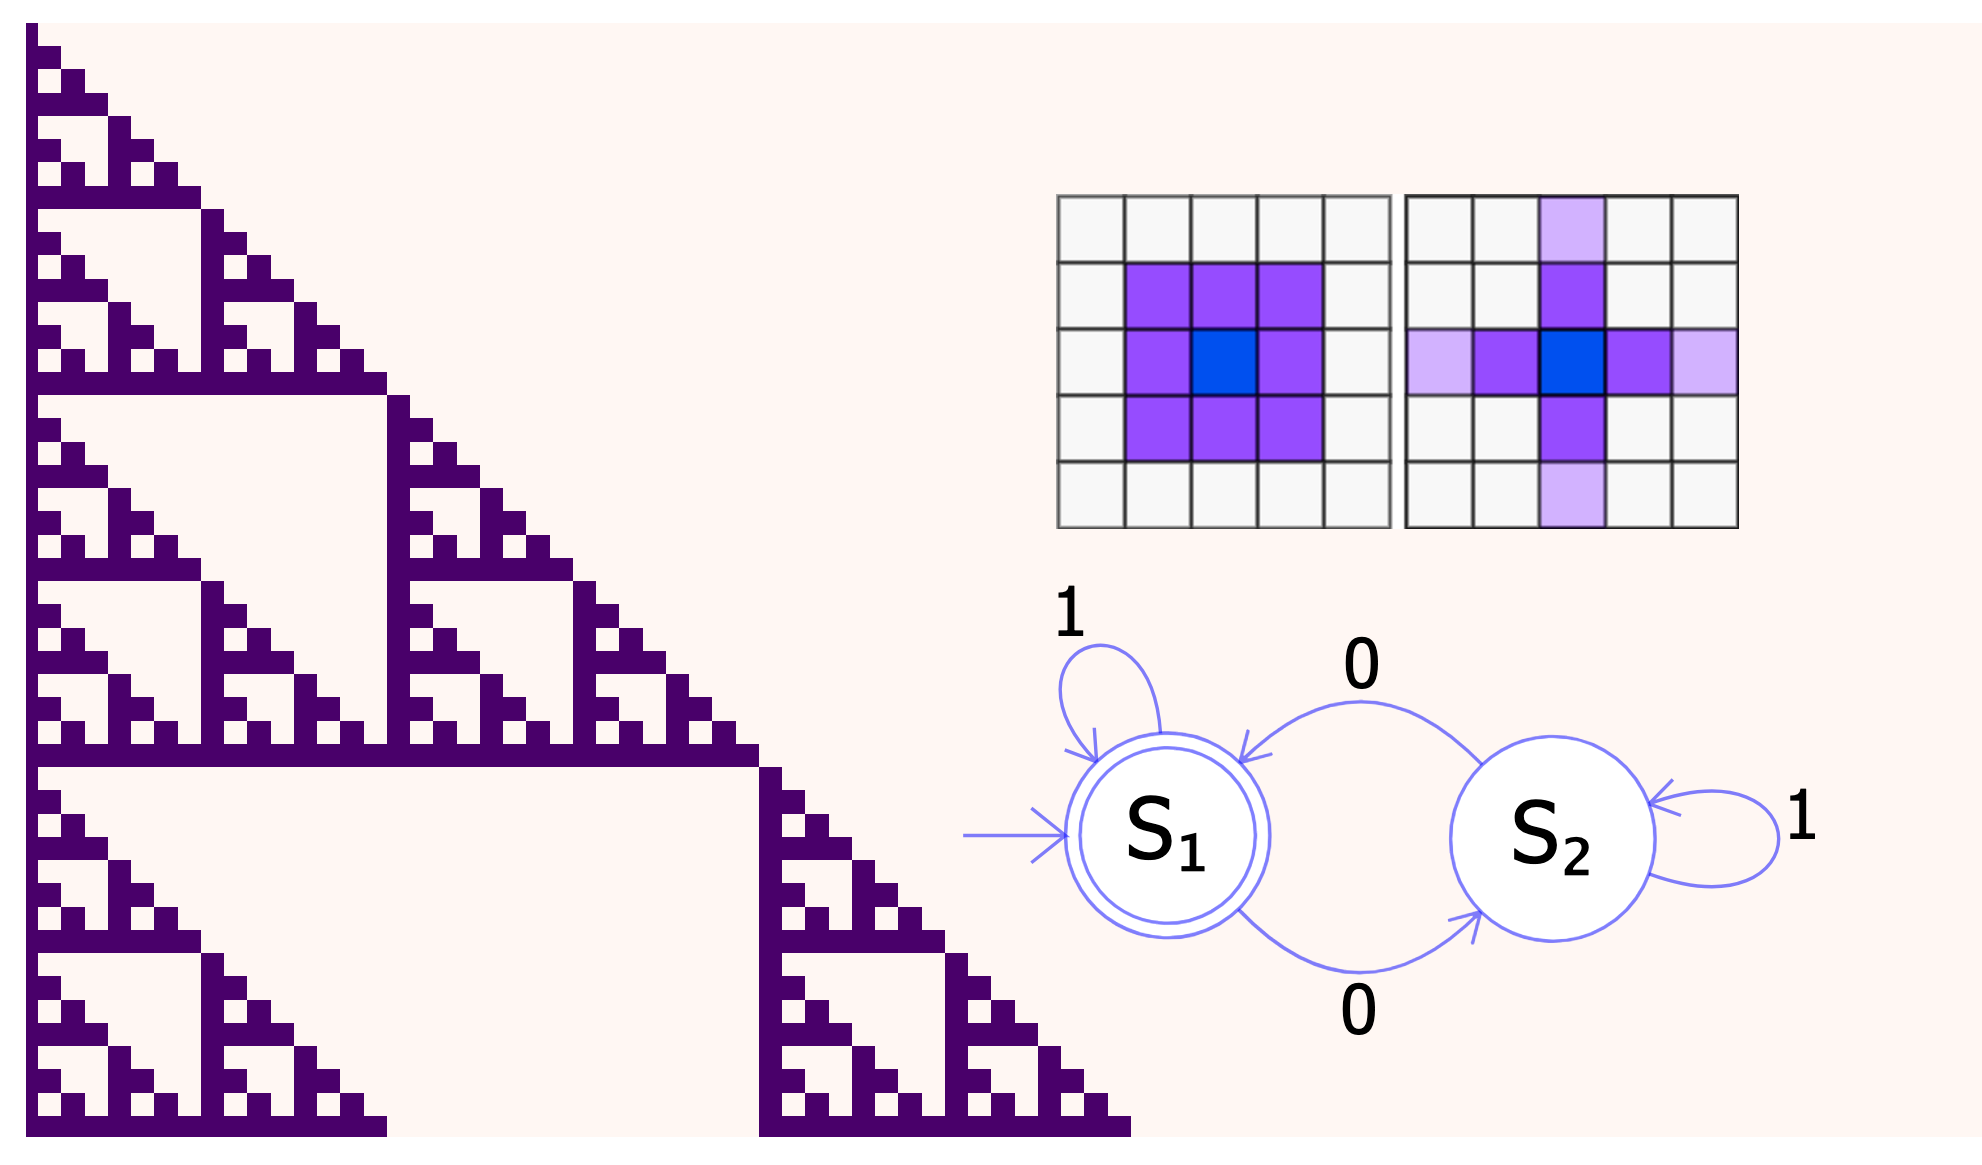
\includegraphics[width=0.75\columnwidth]{figures/theoryOfComputation.png}
		\caption{Example of cellular automata.}
		\label{fig:ExampleAutonoma}
	\end{figure}

\section{Cellular Automata Algorithm}
    \begin{algorithm}
        \caption{Basic Cellular Automaton}
        \KwIn{\texttt{gridWidth}: Width of the grid, \texttt{gridHeight}: Height of the grid, \texttt{states}: Set of possibles states for the cells, \texttt{neighborhood}: Set of relative positions defining the neighborhood of each cell, \texttt{rules}: Set of state transition rules, \texttt{maxTimeSteps}: Maximum number of time steps}
        \KwOut{The final state of the grid}
        
        Initialize \texttt{gridHeight} $\times$ \texttt{gridWidth}, set the initial states on the grid and create \texttt{newGrid} as a copy of the grid.\;
        
        \While{$i$ < \texttt{maxTimeSteps}}{
            \For{$x$ in \texttt{gridWidth}}{
                \For{$y$ in \texttt{gridHeight}}{
                    \texttt{neighbors} = getNeighbors(\texttt{grid}, \texttt{neighborhood}, $x$, $y$)\;
                    \texttt{newGrid}[$x$][$y$] = applyRules(\texttt{grid}[$x$][$y$], \texttt{neighbors}, \texttt{rules})\;
                }
            }
            Display the state of \texttt{newGrid}
            \texttt{grid} = \texttt{newGrid}\;
            $i$++\;
        }
    \end{algorithm}



%%%%%%%%%%%%%%%%%%%%%%%%%%%%%%%%%%%%%%%%%%%%%%%%%%%%%%%%%%%
%%%%%%%%%%%%%%%%%%%%%%%%%%%%%%%%%%%%%%%%%%%%%%%%%%%%%%%%%%%
%%%%%%%%%%%%%%%%%%%%%%%%%%%%%%%%%%%%%%%%%%%%%%%%%%%%%%%%%%%
%%%%%%%%%%%%%%%%%%%%%%%%%%%%%%%%%%%%%%%%%%%%%%%%%%%%%%%%%%%

\section{Parameters Required on a Cellular Automata}

CA, several key parameters need to be defined. These parameters determine the structure, behavior, and evolution of the CA. The primary parameters include:

\subsection{Grid Structure}

\begin{itemize}
    \item \textbf{Dimension:} The number of dimensions of the CA grid. Common configurations are one-dimensional (a line of cells) and two-dimensional (a grid of cells).
    \item \textbf{Size:} The number of cells in each dimension. For example, a one-dimensional CA might have 100 cells, while a two-dimensional CA might have a 100x100 grid.
\end{itemize}

\subsection{Cell States}

\begin{itemize}
    \item \textbf{Number of States:} The finite set of possible states each cell can be in. For example, in a binary CA, each cell can be in one of two states: 0 or 1.
    \item \textbf{Initial Configuration:} The initial state of all cells at time \( t = 0 \). This can be a specific pattern, a random configuration, or any other predefined setup.
\end{itemize}

\subsection{Neighborhood}

\begin{itemize}
    \item \textbf{Radius:} The distance defining the neighborhood of a cell. In a one-dimensional CA, a radius of 1 means the neighborhood includes the cell itself and its immediate left and right neighbors.
    \item \textbf{Shape:} The shape of the neighborhood. Common shapes include the von Neumann neighborhood (cells directly adjacent in cardinal directions) and the Moore neighborhood (cells adjacent in both cardinal and diagonal directions).
\end{itemize}

\subsection{Transition Function}

\begin{itemize}
    \item \textbf{Local Rule:} The function that determines the next state of a cell based on its current state and the states of its neighbors. This function can be deterministic or probabilistic.
    \item \textbf{Update Scheme:} Whether the CA updates all cells simultaneously (synchronously) or one at a time (asynchronously).
\end{itemize}

\subsection{Boundary Conditions}

\begin{itemize}
    \item \textbf{Periodic Boundaries:} Cells at the edge of the grid wrap around to the opposite edge, creating a toroidal structure.
    \item \textbf{Fixed Boundaries:} Cells at the edge of the grid have a fixed state or do not change state based on neighbors outside the grid.
    \item \textbf{Reflective Boundaries:} The states of edge cells are influenced by reflecting the states of neighbors within the grid.
\end{itemize}

\subsection{Time Steps}

\begin{itemize}
    \item \textbf{Discrete Time:} CA evolution occurs in discrete time steps, typically denoted by \( t = 0, 1, 2, \ldots \).
    \item \textbf{Duration:} The number of time steps the CA runs for, which can be predefined or based on a stopping condition.
\end{itemize}

\subsection{Output and Visualization}

\begin{itemize}
    \item \textbf{State Representation:} How the states of the cells are represented visually or numerically (e.g., using different colors or symbols for different states).
    \item \textbf{Data Collection:} Methods for recording the states of cells at each time step for analysis and visualization.
\end{itemize}

By defining these parameters, one can fully specify a Cellular Automaton model and simulate its evolution. The flexibility in choosing these parameters allows CAs to be adapted to a wide range of applications, from simple theoretical models to complex simulations in various fields of science and engineering.



%%%%%%%%%%%%%%%%%%%%%%%%%%%%%%%%%%%%%%%%%%%%%%%%%%%%%%%%%%%
%%%%%%%%%%%%%%%%%%%%%%%%%%%%%%%%%%%%%%%%%%%%%%%%%%%%%%%%%%%
%%%%%%%%%%%%%%%%%%%%%%%%%%%%%%%%%%%%%%%%%%%%%%%%%%%%%%%%%%%
%%%%%%%%%%%%%%%%%%%%%%%%%%%%%%%%%%%%%%%%%%%%%%%%%%%%%%%%%
\section{Versions of Cellular Automata}
CA have evolved into various versions and classifications based on their dimensionality, state complexity, neighborhood structure, and rule sets. Here are some of the key versions of Cellular Automata:

\subsection{By Dimensionality}

\begin{itemize}
    \item \textbf{One-Dimensional Cellular Automata:} Each cell has two neighbors (left and right). These are the simplest form and are often used for theoretical studies. An example is the elementary cellular automata defined by Stephen Wolfram.
    \item \textbf{Two-Dimensional Cellular Automata:} Each cell has multiple neighbors depending on the neighborhood structure. Conway's Game of Life is a well-known example.
    \item \textbf{Higher-Dimensional Cellular Automata:} These include three-dimensional and higher-dimensional grids, which are used for more complex simulations but are less common due to increased computational complexity.
\end{itemize}

\subsection{By Cell States}

\begin{itemize}
    \item \textbf{Binary Cellular Automata:} Each cell can be in one of two states, typically denoted as 0 and 1. This is the simplest form and is widely studied.
    \item \textbf{Multi-State Cellular Automata:} Cells can exist in more than two states. These automata are used to model more complex systems where each cell can represent multiple possible conditions.
    \item \textbf{Continuous-State Cellular Automata:} Cells can take on a range of continuous values, rather than discrete states, allowing for the modeling of more nuanced phenomena.
\end{itemize}

\subsection{By Neighborhood Type}

\begin{itemize}
    \item \textbf{Von Neumann Neighborhood:} Consists of the four orthogonal neighbors (north, south, east, and west) of a cell in a two-dimensional grid.
    \item \textbf{Moore Neighborhood:} Includes the eight surrounding cells (both orthogonal and diagonal neighbors) in a two-dimensional grid.
    \item \textbf{Extended Neighborhoods:} Larger neighborhoods that include more distant neighbors, such as the Margolus neighborhood.
\end{itemize}

\subsection{By Rule Type}

\begin{itemize}
    \item \textbf{Deterministic Cellular Automata:} The next state of each cell is determined entirely by the current state and the states of its neighbors, following a fixed rule.
    \item \textbf{Probabilistic Cellular Automata:} The next state of each cell is determined probabilistically, allowing for the modeling of stochastic processes.
    \item \textbf{Totalistic Cellular Automata:} The state of a cell depends only on the total number (or sum) of particular states in the neighborhood, not on the exact configuration of those states.
\end{itemize}

\subsection{By Boundary Conditions}

\begin{itemize}
    \item \textbf{Periodic Boundary Conditions:} The grid is treated as if it wraps around on itself, creating a toroidal structure.
    \item \textbf{Fixed Boundary Conditions:} The states of the cells at the boundaries are fixed and do not change.
    \item \textbf{Reflective Boundary Conditions:} The states of the cells at the boundaries reflect the states of their neighbors inside the grid.
\end{itemize}

\subsection{Special Types of Cellular Automata}

\begin{itemize}
    \item \textbf{Elementary Cellular Automata:} A class of one-dimensional binary cellular automata defined by Stephen Wolfram, consisting of 256 possible rules.
    \item \textbf{Conway's Game of Life:} A two-dimensional binary cellular automaton devised by John Conway, famous for its simple rules leading to complex behavior.
    \item \textbf{Langton's Ant:} A two-dimensional Turing machine with very simple rules but complex emergent behavior.
    \item \textbf{Fuzzy Cellular Automata:} Combines cellular automata with fuzzy logic to handle uncertainty and imprecision in state transitions.
    \item \textbf{Quantum Cellular Automata:} An extension of cellular automata principles to quantum computing, allowing cells to be in superpositions of states.
\end{itemize}

These different versions of cellular automata enable the modeling and simulation of a wide range of systems, from simple theoretical constructs to complex real-world phenomena.


%%%%%%%%%%%%%%%%%%%%%%%%%%%%%%%%%%%%%%%%%%%%%%%%%%%%%%%%%%%
%%%%%%%%%%%%%%%%%%%%%%%%%%%%%%%%%%%%%%%%%%%%%%%%%%%%%%%%%%%
%%%%%%%%%%%%%%%%%%%%%%%%%%%%%%%%%%%%%%%%%%%%%%%%%%%%%%%%%%%
%%%%%%%%%%%%%%%%%%%%%%%%%%%%%%%%%%%%%%%%%%%%%%%%%%%%%%%%%
\section{Analogy with the Nature}
    
CA come in various forms, each inspired by different aspects of natural systems. These versions differ based on their dimensionality, complexity, neighborhood structure, and the rules that govern them.

\subsection{Dimensionality}

Just as nature operates at different scales, from the linear growth of a vine to the branching of trees and the intricate structures of coral reefs, CAs can also be one-dimensional, two-dimensional, or even higher-dimensional. One-dimensional CAs, like a line of ants following each other, are the simplest and often used for theoretical studies \cite{wolfram2002}. Two-dimensional CAs resemble the spread of moss on a rock surface, where each cell interacts with its immediate neighbors in a grid pattern \cite{gardner1970}. Higher-dimensional CAs, though more complex, can model phenomena such as the three-dimensional growth of crystals or the propagation of signals in a neural network.

\subsection{Cell States}

In the same way that an organism can be alive or dead, hibernating or active, cells in a CA can exist in various states. Binary CAs, where each cell can be either 0 or 1, are analogous to on/off states, such as a plant being either alive or dead. Multi-state CAs extend this analogy by allowing for intermediate states, similar to a tree showing different stages of leaf growth, colors, and shedding. Continuous-state CAs go even further, representing states on a spectrum, akin to the varying shades of green in a forest canopy.

\subsection{Neighborhoods}

The interactions in nature are often local. A tree might only affect and be affected by the trees around it. Similarly, in a CA, the concept of a neighborhood defines which cells influence a given cell's state. In a von Neumann neighborhood, a cell's state is influenced by its four orthogonal neighbors, like a central plant interacting with the four closest plants around it. In a Moore neighborhood, the interaction extends to include diagonal neighbors as well, resembling a plant affected by all surrounding plants in a 3x3 grid.

\subsection{Rule Types}

The rules that govern a CA's evolution can be deterministic or probabilistic, mirroring the predictability or randomness found in nature. Deterministic CAs follow fixed rules, much like the consistent seasonal changes that influence plant growth. Probabilistic CAs, on the other hand, incorporate randomness, similar to how weather patterns can unpredictably affect an ecosystem. Totalistic CAs simplify these interactions by considering the sum of states in the neighborhood, analogous to how the overall density of a forest might influence the growth of an individual tree rather than the specific arrangement of nearby trees.

\subsection{Boundary Conditions}

Nature often operates within boundaries, such as the edge of a forest or the banks of a river. In CAs, boundary conditions define the limits of the grid. Periodic boundaries wrap around, creating a seamless, toroidal structure, similar to the cyclical nature of seasons or life cycles. Fixed boundaries impose a rigid edge, like the shorelines of an island. Reflective boundaries mimic natural barriers that reflect influence, akin to a mountain reflecting sound waves.

\subsection{Special Types of Cellular Automata}

Several special types of CAs draw direct analogies from natural phenomena. Elementary Cellular Automata, defined by Stephen Wolfram, explore simple, one-dimensional rules that can lead to complex behavior \cite{wolfram2002}, much like simple genetic rules can lead to diverse biological traits. Conway's Game of Life, a two-dimensional CA, mirrors the lifecycle of organisms with birth, survival, and death rules, showing how simple interactions can create complex, lifelike patterns \cite{gardner1970}. Langton's Ant is an example of how simple local rules can produce unexpected, emergent behavior, similar to how individual ant movements result in organized colony paths \cite{langton1986}.

Fuzzy Cellular Automata combine CA principles with fuzzy logic to handle uncertainty \cite{pedrycz2010}, much like how plants might adapt their growth based on varying environmental conditions rather than strict rules. Quantum Cellular Automata extend these concepts into the quantum realm, where cells can exist in superpositions of states, analogous to quantum particles exhibiting multiple states simultaneously \cite{brennen2003}.

These diverse versions of Cellular Automata reflect the richness and variety found in natural systems, allowing for the modeling and simulation of both simple and complex phenomena across different fields of study.

%%%%%%%%%%%%%%%%%%%%%%%%%%%%%%%%%%%%%%%%%%%%%%%%%%%%%%%%%%%
%%%%%%%%%%%%%%%%%%%%%%%%%%%%%%%%%%%%%%%%%%%%%%%%%%%%%%%%%%%
%%%%%%%%%%%%%%%%%%%%%%%%%%%%%%%%%%%%%%%%%%%%%%%%%%%%%%%%%%%
%%%%%%%%%%%%%%%%%%%%%%%%%%%%%%%%%%%%%%%%%%%%%%%%%%%%%%%%%


%%%%%%%%%%%%%%%%%%%%%%%%%%%%%%%%%%%%%%%%%%%%%%%%%%%%%%%%%%%
%%%%%%%%%%%%%%%%%%%%%%%%%%%%%%%%%%%%%%%%%%%%%%%%%%%%%%%%%%%
%%%%%%%%%%%%%%%%%%%%%%%%%%%%%%%%%%%%%%%%%%%%%%%%%%%%%%%%%%%
%%%%%%%%%%%%%%%%%%%%%%%%%%%%%%%%%%%%%%%%%%%%%%%%%%%%%%%%%
\section{Usage Examples}
In the following section, we present some articles where you can find implementations of cellular automata.

\subsection{ A computational tumor growth model experience based on molecular dynamics point of view using deep cellular automata }

The article \textit{A computational tumor growth model experience based on molecular dynamics point of view using deep cellular automata} discusses a novel approach to modeling cancerous tumor growth by integrating cellular automata (CA) with deep learning techniques, particularly convolutional neural networks (CNNs). This integration aims to leverage the strengths of both methods to create a robust and scalable solution for simulating tumor development.\cite{MATIN2024102752}

\subsubsection{Overview of Cellular Automata and CNN Integration}

Cellular automata are dynamic systems composed of a grid of cells, each of which can be in one of several states. The state of each cell at any given time is determined by a set of rules that consider the states of neighboring cells. Traditional CA models operate based on predetermined rules, which can be rigid and may not adapt well to varying conditions. By contrast, when CA rules are implemented within a CNN framework, these rules can potentially be learned from data, making the system adaptive and capable of handling more complex and varied scenarios.

\subsubsection{Implementation Details}

The article details how the CA is represented as a CNN. The process involves defining the CA as a mapping between possible pixel configurations in a binary image and corresponding output pixel values. This mapping is applied to randomly generated binary images to create training data, which are then used to train the CNN. The network architecture typically involves a 3 $×$ 3 convolution layer followed by several 1 $×$ 1 convolution layers. This setup allows the network to perform local operations repeatedly, mimicking the behavior of CA.

The integration of CA with CNNs provides several advantages:

\begin{itemize}
    \item \textbf{Scalability}: Leveraging the parallel processing capabilities of modern GPUs optimized for CNN operations allows for faster simulations and predictions, especially for large grid sizes.
    \item \textbf{Granular Predictions}: By integrating CA rules within a CNN framework, it is possible to achieve detailed predictions at the cellular level. This granularity is crucial for applications like tumor growth prediction, where understanding cellular interactions at a micro-level can provide invaluable insights.
    \item \textbf{Adaptability}: Unlike traditional CA models that are constrained by predefined rules, the CNN-based approach allows for the rules to be learned from data, enhancing the system's ability to generalize and adapt to different conditions.
\end{itemize}

\subsubsection{Results and Validation}

The proposed model was validated by comparing its output to established mathematical models of tumor growth, specifically the Gompertz growth model. The results showed that the CNN-CA model aligns well with the Gompertz model, demonstrating its accuracy and robustness. Additionally, the model was tested on various tumor growth datasets, highlighting its versatility and predictive capabilities.

This research paves the way for more sophisticated and adaptable models in the field of tumor growth simulation, offering a promising direction for future studies in oncology.

\subsection{Implementing Fuzzy Cellular Automata in Breast Cancer Image Segmentation}

The article \textit{Breast Cancer Images Segmentation using Fuzzy Cellular Automaton} presents an innovative approach for segmenting breast cancer images by integrating Cellular Automata (CA) with Fuzzy Logic, resulting in the so-called Fuzzy Cellular Automaton. This method aims to enhance the accuracy and flexibility of segmenting the mass region in mammograms, achieving highly promising results with an accuracy of 98.66\% on the mini-MIAS dataset.\cite{ION2023999}

\subsubsection{Overview of Cellular Automata and Fuzzy Logic Integration}

Cellular Automata (CA) are dynamic systems comprised of a grid of cells, each of which can be in one of several states. The state of each cell at any given time is determined by a set of rules that consider the states of neighboring cells. Traditional CA models operate based on predetermined rules, which can be rigid and may not adapt well to varying conditions. By incorporating Fuzzy Logic into CA, the model gains the ability to categorize pixels more flexibly, enhancing its adaptability to different imaging scenarios.

\subsubsection{Implementation Details}

The article outlines how CA is combined with Fuzzy Logic to form a Fuzzy Cellular Automaton. This process involves several key steps:

\begin{enumerate}
    \item \textbf{Preprocessing}: The mammogram images are converted to grayscale, and noise is reduced using Gaussian Blur and Binary Threshold techniques. Background and pectoral muscle removal are performed to isolate the region of interest (ROI).

    \item \textbf{Segmentation}: An improved version of the CA algorithm is applied to the preprocessed images. The segmentation starts with a pixel (seed) and expands to neighboring pixels with similar shades, computing the strength of the neighboring cells based on the CA rules. 

    \item \textbf{Fuzzy Logic Integration}: To refine the segmentation, Fuzzy Logic is applied. Two fuzzy sets are constructed based on the grayscale distributions of the strength determined by the CA algorithm. These sets model the presence of a certain pixel in the suspicious region and the contrary event.
\end{enumerate}

\subsubsection{Advantages of the Approach}

Integrating CA with Fuzzy Logic offers several advantages:

\begin{itemize}
    \item \textbf{Improved Accuracy}: The method achieves a high accuracy rate of 98.66\% on the mini-MIAS dataset, significantly improving the precision of mass region segmentation.
    \item \textbf{Flexibility}: Fuzzy Logic provides a more adaptable technique for pixel categorization, allowing the model to handle variations in imaging conditions more effectively.
    \item \textbf{Visual Clarity}: The visually progressive nature of CA, combined with the adaptability of Fuzzy Logic, results in clearer and more interpretable segmentation results for medical specialists.
\end{itemize}

\subsubsection{Experimental Results}

The proposed approach was validated on the mini-MIAS dataset, comprising 322 mammograms, 118 of which contain suspicious masses. The results showed that the Fuzzy Cellular Automaton outperformed the traditional CA approach, with a mean Intersection over Union (IoU) score of 83.79\%, compared to 65.11\% for the CA approach.


%%%%%%%%%%%%%%%%%%%%%%%%%%%%%%%%%%%%%%%%%%%%%%%%%%%%%%%%%%%
%%%%%%%%%%%%%%%%%%%%%%%%%%%%%%%%%%%%%%%%%%%%%%%%%%%%%%%%%%%
%%%%%%%%%%%%%%%%%%%%%%%%%%%%%%%%%%%%%%%%%%%%%%%%%%%%%%%%%%%

\section{Implementation Repositories}

In this section, we present some repositories where you can find implementations of cellular automata.

\subsection*{Sandspiel}
Made by Max Bittker, Sandspiel is a falling sand game that provides a creative and interactive environment for exploring cellular automata. Users can experiment with different elements, such as sand, water, fire, and plants, and observe how they interact and evolve over time. Sandspiel is available online and offers a user-friendly interface for designing and simulating complex cellular automata systems.

You can access the repository at: \url{https://github.com/MaxBittker/sandspiel}
\subsection*{terra}
JS library for cellular automata and simple biological simulations. textit{Terra} provides a flexible and extensible framework for creating and simulating cellular automata models. It includes various built-in rules and configurations for different types of automata, making it easy to experiment with different systems and behaviors. terra is designed to be user-friendly and accessible for both beginners and advanced users.

You can access the repository at: \url{https://rileyjshaw.com/terra/}
\section{Conclusion}
In this paper, we have explored the concept of Cellular Automata (CA) and its various types, including deterministic and probabilistic CAs. We have also discussed the importance of boundary conditions in CA models and highlighted some special types of CAs that draw analogies from natural phenomena.

Furthermore, we have presented two usage examples of CA in different domains. The first example demonstrates the integration of CA with deep learning techniques for modeling tumor growth, showcasing the scalability and adaptability of the approach. The second example showcases the integration of CA with fuzzy logic for breast cancer image segmentation, highlighting the improved accuracy and visual clarity achieved through this integration.

Overall, Cellular Automata provide a powerful framework for modeling and simulating complex phenomena in various fields. The versatility and adaptability of CA make it a valuable tool for understanding and analyzing natural systems. With further research and development, CA-based models can contribute to advancements in fields such as biology, medicine, and environmental science.

In conclusion, Cellular Automata offer a promising avenue for studying and simulating both simple and complex phenomena, providing insights into the dynamics of natural systems and enabling the development of innovative solutions in various domains.

\printbibliography

\end{document}